\documentclass[12pt]{article}
\usepackage{graphicx}
\usepackage{amsmath}

\begin{document}

\section{Figure}
I took some beautiful pictures. Figure \ref{fig:lapic} shows what you want to see.

\begin{figure}[htb]
\centering
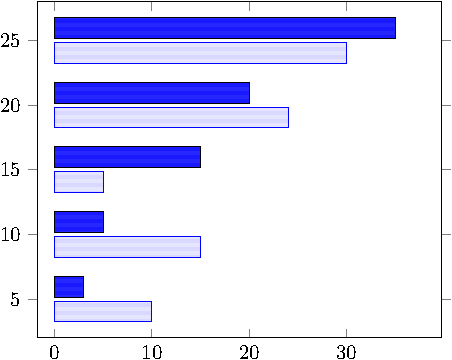
\includegraphics[scale=0.7]{fig1}
\caption{This is my first latex picture}\label{fig:lapic}
\end{figure}

\section{Table}

Table \ref{tab:example}.

\begin{table}[!htb]
\centering
\caption{A example of table}\label{tab:example}
\begin{tabular}{|c|c|c|c|}
\hline 
a & b & c & d\\
\hline 
1 & 2 & 3 & 4 \\
\hline 
5 & 6 & 7 & 8 \\
\hline 
\end{tabular}
\end{table}



\numberwithin{table}{section}
\begin{table}[!htb]
\centering
\caption{A example of table}\label{tab:example2}
\begin{tabular}{|c|c|c|c|}
\hline 
a & b & c & d\\
\hline 
1 & 2 & 3 & 4 \\
\hline 
5 & 6 & 7 & 8 \\
\hline 
\end{tabular}
\end{table}

\end{document}
